\chapter{Attention, Leverage, and the Creator Machine}

This School of Hard Knocks interview, curated by LazyingArt LLC, is not a blackboard lecture in the usual sense. Its mathematics is the mathematics of commercial conversion: attention into audience, audience into revenue, bargaining position into leverage, and cash income into ownership. The host begins with scale---a young creator, a best year a little above \$30 million, a mansion above \$25 million---and then deliberately delays the main case. We first gather an older grammar of sales and capital in Miami, and only afterward return to Adin Ross to see how the creator economy rearranges those older rules.

\section{Scale Before Mechanism}

The opening move is simple and effective. We are not first given a theory; we are given magnitude. The lecture announces a 24-year-old creator, a best year a little above \$30 million, and a house priced in the neighborhood of \$25 million. Only after the numbers have done their work does the host ask the real question: how does somebody become wealthy in this world?

We may compress the opening numerical anchors as
\begin{equation}
a = 24,\qquad Y_{\max} > \$30\,\mathrm{M},\qquad P_{\text{house}} \approx \$25.5\,\mathrm{M}.
\end{equation}
These are not yet explanations. They are the boundary conditions of the problem.

What matters next is the delay. The lecture does not move directly from spectacle to explanation. Instead it detours through Miami's Design District, as if to say that before we understand a modern creator fortune we should first hear the older commercial doctrines out of which such a fortune is still partly built. In this respect the opening is pedagogically sound: scale creates curiosity, but the explanation is postponed until we have assembled some machinery.

\section{Miami Prelude I: Closing the Sale}

Before meeting Ross, the host uses his own public reach as a passport. Even the cold approach has economic content, since audience size functions as credibility and access:
\begin{equation}
N_{\text{host}} \approx 15 \times 10^6.
\end{equation}
This is a small version of the larger thesis that will come later. Attention already buys something.

The first Miami operator then gives the lecture its earliest durable rules. He made money in real estate development, had a very large year, and compresses his doctrine into a few sentences: wrap the sale, do not talk past the sale, do not negotiate against yourself, and listen more than you speak. We may write the listening heuristic as
\begin{equation}
\text{listening} : \text{talking} \approx 2:1.
\end{equation}

If we formalize his sales view only as much as the lecture supports, we get two compact relations:
\begin{align}
\mathbb{E}[S] &= np,\\
c \uparrow &\Rightarrow p_{\text{close}}(c)\downarrow.
\end{align}
Here \(n\) is the number of qualified encounters, \(p\) the probability of closing one of them, and \(c\) the buyer confusion introduced after intent has already formed. The first line is his ``sales is statistical'' claim. The second is the shoe-store story in compressed form: once a buyer is ready, extra options need not increase value; they may instead reduce the chance of finishing the transaction.

\subsection{Question \& Answer}

Why can talking after the sale has essentially happened still destroy the sale?

Because at that moment the limiting factor is no longer awareness. The buyer already has intent. The danger is that the salesperson reopens the decision and converts commitment into comparison. In the lecture's language, five new pairs of shoes are not five new opportunities; they are five new ways to leave empty-handed. The close is therefore not improved by endless elaboration. It is often improved by silence, paperwork, and exit.

The operator's biography gives this advice some weight. He says he moved to California young, entered commission-only work, ran out of money, and was sent back out by his father with just enough to try again. He hated sales, but had to do it. That matters. The lecture is not sentimental here. Selling is treated less as charisma than as repetition under pressure. From that point of view the closing maxim,
\[
\text{see the guy} \to \text{ask him to buy},
\]
is not decorative. It is the operational corollary of \(\mathbb{E}[S]=np\).

\section{Miami Prelude II: Access, Cash, and Time Horizon}

The second Miami operator changes the tone. He manages a very large pool of money, but he does not present a clean bootstrap story. He says plainly that he did not begin from nothing and that some wealthy relationships are inherited through school, family, and circle. The lecture is stronger when it leaves that tension visible. Not all access is earned in the same way.

The capital-allocation grammar here is also different. The emphasis is not on closing a sale but on preserving room to act. The interviewer's questions draw out several distinct positions:
\begin{itemize}
\item some networks are pre-existing rather than constructed from scratch;
\item defensive cash is valuable in uncertain periods;
\item a smaller outsider sum, around \$100{,}000, is directed toward a mutual fund rather than a heroic concentrated bet;
\item single-family real estate is praised as a long-hold asset rather than a quick flip;
\item the claims about gold, Buffett-like cash posture, and timing the next purchase should be read as interview material, not as settled doctrine.
\end{itemize}

The structural lesson is nevertheless clear. The operator prefers optionality. Dry powder today is presented as buying room tomorrow. That is a different wealth grammar from the first Miami case, but not an unrelated one. In both cases the central object is freedom of action: in sales, freedom to close without confusion; in capital markets, freedom to wait without being forced.

\paragraph{A brief sponsor hinge.} The sponsor interlude is not central doctrine, but it serves a structural purpose. The host says that rich operators are unusually clear communicators. Even when we compress the advertisement, we should keep that hinge, because it bridges the street interviews and the mansion interview. The transition claim is that clarity helps convert access into deals, and deals into money.

\section{Self-Worth and Walk-Away Leverage}

When the lecture finally arrives at Ross's house, it does not begin with platform economics. It begins with family doubt, paternal support, early streaming infrastructure, and then betrayal in business. That order matters. Before Ross explains monetization, he explains posture.

His account is straightforward. Many doubted him. His father did not. The father believed early enough to fund the practical conditions of the bet, even down to better internet. That story is immediately followed by the claim that people will repeatedly take from you until you understand your own value. Self-worth is therefore not presented as therapy-talk. It is a commercial boundary.

We can formalize Ross's bargaining claim in the mildest possible way:
\begin{proposition}
In the bargaining grammar of the lecture, leverage rises with outside options and with genuine willingness to walk away:
\begin{equation}
L = L(O,w),\qquad \frac{\partial L}{\partial O}>0,\qquad \frac{\partial L}{\partial w}>0.
\end{equation}
\end{proposition}

\begin{proof}
If a negotiator can actually leave, then ``no deal'' is a live outcome rather than a bluff. The counterparty must price that possibility. Ross states the result verbally: the person with the most leverage is the one most willing to walk away.
\end{proof}

\subsection{Question \& Answer}

Why is willingness to walk away the source of leverage?

Because business bargaining is full of staged confidence. If both sides talk as though they can leave, but only one side actually can, then only one side possesses a credible threat. The lecture makes the point in ordinary language: people bluff, politics enters, appearances are managed. Under those conditions, a real outside option is worth more than a loud declaration. Ross even says he has missed multimillion-dollar opportunities by walking away, but the lecture presents those misses not as losses in a narrow sense. They are the price paid for keeping the right to say no, and that right later yields different deals on different terms.

The chapter should also keep the connection between self-worth and leverage visible. A person who does not believe in his own replaceability, or in his own ability to begin again elsewhere, will find it difficult to set \(w\) high enough for the proposition above to matter. The willingness to walk is not only financial. It is psychological.

\section{Attention, Loyalty, and the Revenue Machine}

Once leverage is on the table, the lecture moves to its central economic claim. Ross is asked about the biggest year of his career and again gives a number a little above \$30 million. But the interesting part is not the total. The interesting part is the explanation. He does not say merely that he streamed. He says he has people who watch him daily, who are not just followers but something closer to family. The host then supplies the compressed business slogan: where attention goes, revenue flows.

We may state the lecture's main mechanism as a definition.

\begin{definition}
The creator machine of the lecture is the chain
\begin{equation}
A \to B \to R,
\end{equation}
where \(A\) denotes attention, \(B\) a loyal audience base, and \(R\) monetized revenue.
\end{definition}

This is a sharper object than generic ``content creation.'' The host even reinforces the point by recalling Ryan Serhant's remark that the decisive skill is no longer merely selling well, but getting attention in the first place. That is why the Miami prelude belongs here. The first operator taught us how to close. Ross and the host now argue that before closing comes capture.

Once the base \(B\) is established, the revenue channels can be written schematically as
\begin{equation}
R = R_{\text{subs}} + R_{\text{tips}} + R_{\text{KCIP}} + R_{\text{brand}} + R_{\text{equity}}.
\end{equation}
The lecture does not present this formula explicitly, but it is the cleanest way to hold together the monetization channels Ross names later: subscriptions, tip-like donations, platform income, brand deals, and ownership positions.

Ross's other great claim in this middle part is about fear. He says that what separated him was not fearing, and he uses the house itself as an example of a larger policy: pull the trigger, accept that consequences come later, and learn through contact rather than hesitation. The danger of this rhetoric is obvious if stated without restraint. Yet inside the lecture it plays a precise role. It is the bridge from attention to deployment. One first builds a loyal base, and then one uses the resulting cash flow and confidence to act.

\section{Ownership, Clip Funnels, and Platform Pay}

The lecture now turns from earning money to placing it. Ross lists crypto, real estate, watches, and stocks, while warning against greed in volatile markets. The most compact expression of his crypto rule is simply this:
\begin{equation}
m\in\{1.5,2\}\ \text{may be enough; do not wait greedily for }m=10.
\end{equation}
Here \(m\) is the gross return multiple on a position. We should not over-theorize the remark. It is not investment doctrine; it is a rule of temperament. Take profit, keep cash, and do not assume the market owes you the next multiple.

From there the lecture makes a more durable shift. Ross says that the truly important thing is not quick cash but equity. In notation:
\begin{equation}
C \quad \text{versus} \quad \alpha V.
\end{equation}
A cash deal gives immediate fixed value \(C\). An ownership share gives \(\alpha V\), a fraction of future firm value. Ross's point is that if the platform grows large enough, \(\alpha V\) dominates the short cash payment. This is why he says ownership is king. Control and upside sit in the same place.

\subsection{Question \& Answer}

How does a 10--30 second clip become money?

Not by being the final product. The clip is a transport mechanism. The long stream contains the full event; the clip extracts the moment with the highest shareability; the shared moment redirects attention back to the live stream or the creator's broader ecosystem; only then do the monetization channels switch on. The short clip is therefore not a substitute for the main act. It is a funnel into the main act.

We can display the process as a schematic figure.

\begin{figure}
\centering
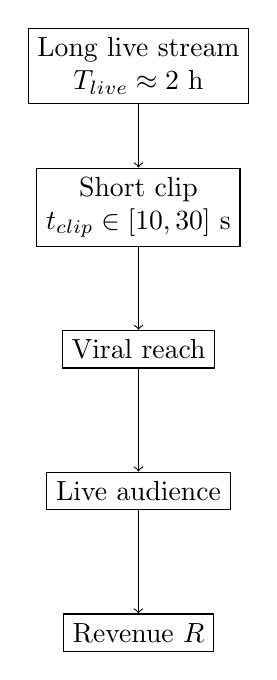
\begin{tikzpicture}[x=1cm,y=1cm]
\node[draw, align=center] (live) at (0,0) {Long live stream\\$T_{\text{live}}\approx 2$ h};
\node[draw, align=center] (clip) at (0,-1.8) {Short clip\\$t_{\text{clip}}\in[10,30]$ s};
\node[draw, align=center] (reach) at (0,-3.6) {Viral reach};
\node[draw, align=center] (aud) at (0,-5.4) {Live audience};
\node[draw, align=center] (rev) at (0,-7.2) {Revenue $R$};
\draw[->] (live) -- (clip);
\draw[->] (clip) -- (reach);
\draw[->] (reach) -- (aud);
\draw[->] (aud) -- (rev);
\end{tikzpicture}
\end{figure}

In symbols, the same chain is
\begin{equation}
\text{live stream} \to \text{clip} \to \text{viral reach} \to \text{live viewers} \to R.
\end{equation}

The lecture then becomes unusually concrete. Ross gives platform heuristics for Kik:
\begin{equation}
r_h(100) \approx \$7\text{--}8/\text{hr},\qquad
r_h(1000) \approx \$100\text{--}200/\text{hr}.
\end{equation}
These are spoken examples, not a law of motion, but they are useful because they reveal the lecture's desire to move from glamour back to arithmetic.

\paragraph{A worked arithmetic example.} Ross says that in June he completed \(18\) streams and made \$623{,}000 through the relevant platform program. The rough average per paid stream is therefore
\begin{align}
N_{\text{streams}} &= 18,\\
R_{\text{June}} &= \$623{,}000,\\
\bar R_{\text{stream}}
&\approx \frac{R_{\text{June}}}{N_{\text{streams}}}
= \frac{623{,}000}{18}
\approx \$34{,}611.
\end{align}
We should keep this arithmetic in perspective. It is only a coarse average. It does not tell us how long each stream lasted, how variable the audience was, or how much additional income was arriving from other channels. Still, it is the lecture's clearest moment of explicit numerical mechanism.

The closing advice returns to temperament. Ross admits luck in streaming, insists that people may look crazy before they look brilliant, and then gives the most concrete of his final rules:
\begin{equation}
T_{\text{focus}} = 1\ \text{year}.
\end{equation}
Focus on one thing for a full year, even while holding a regular job. This is less precise than the monetization arithmetic, but it is not empty. The lecture ends by folding luck, persistence, and concentration into one final discipline: keep the experiment alive long enough for the machine to compound.

\section{Summary}

The lecture begins with spectacle and earns its way back to mechanism. Miami supplies the older doctrine: close the sale, do not negotiate against yourself, preserve optionality, and think in long horizons. Ross then translates that grammar into a creator economy: attention first, loyalty second, revenue third. From there the machine broadens into ownership. Cash matters, but equity matters more; clips matter, but only as funnels; confidence matters, but only when it becomes a credible willingness to walk away or a sustained willingness to keep building.

If we compress the whole chapter into one line, it is this:
\[
\text{attention} \to \text{audience} \to \text{cash flow} \to \text{ownership} \to \text{further optionality}.
\]
That chain is the real subject of the interview.